\documentclass[tikz,margin=2mm]{standalone}
\usepackage{tikz}
\begin{document}
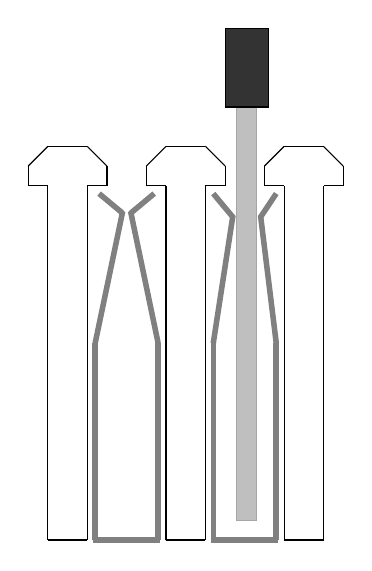
\begin{tikzpicture}[x=5mm,y=5mm]

  \foreach \x in {1,4,7}{
    \draw[color=black] (\x + 0.5,00.0) -- (\x + 1.5,00.0);
    \draw[color=black] (\x + 0.5,00.0) -- (\x + 0.5,09.0);
    \draw[color=black] (\x + 0.5,09.0) -- (\x + 0.0,09.0);
    \draw[color=black] (\x + 0.0,09.0) -- (\x + 0.0,09.5);
    \draw[color=black] (\x + 0.0,09.5) -- (\x + 0.5,10.0);
    \draw[color=black] (\x + 0.5,10.0) -- (\x + 1.5,10.0);
    \draw[color=black] (\x + 1.5,10.0) -- (\x + 2.0,09.5);
    \draw[color=black] (\x + 2.0,09.5) -- (\x + 2.0,09.0);
    \draw[color=black] (\x + 2.0,09.0) -- (\x + 1.5,09.0);
    \draw[color=black] (\x + 1.5,09.0) -- (\x + 1.5,00.0);
  }
  
  \draw[color=gray, line width=2] (2.80,08.80) -- (3.40,08.30);
  \draw[color=gray, line width=2] (3.40,08.35) -- (2.70,05.00);
  \draw[color=gray, line width=2] (4.20,08.80) -- (3.60,08.30);
  \draw[color=gray, line width=2] (3.60,08.35) -- (4.30,05.00);
  \draw[color=gray, line width=2] (2.70,00.00) -- (2.70,05.00);
  \draw[color=gray, line width=2] (2.65,00.00) -- (4.35,00.00);
  \draw[color=gray, line width=2] (4.30,00.00) -- (4.30,05.00);
  
  \draw[color=gray, line width=2] (5.70,08.80) -- (6.20,08.20);
  \draw[color=gray, line width=2] (6.20,08.25) -- (5.70,05.00);
  \draw[color=gray, line width=2] (7.30,08.80) -- (6.90,08.20);
  \draw[color=gray, line width=2] (6.90,08.25) -- (7.30,05.00);
  \draw[color=gray, line width=2] (7.30,00.00) -- (7.30,05.00);
  \draw[color=gray, line width=2] (5.65,00.00) -- (7.35,00.00);
  \draw[color=gray, line width=2] (5.70,00.00) -- (5.70,05.00);  
  
  \draw[color=gray!70, fill=gray!50] (6.30,0.50) rectangle (6.8,11.0);
  \draw[color=black, fill=black!80] (6.00,11.00) rectangle (7.1,13.00);
\end{tikzpicture}
\end{document}